\section{Chapter 3 Steam Generation \& Distribution}
\subsection{Steam Generation}
Steam generation is the process of producing steam from water. The steam generation process involves several steps, from water intake to the final production of high-pressure steam. Below is an overview of the typical steam generation that is done through the application of heat:

\textbf{1. Water Intake:} The process begins with the intake of water from a natural source, such as a river, lake, or reservoir. 

\textbf{2. Water Treatment:} In industrial application in order to ensure the efficient and safe operation of the steam generation system, the water must undergo treatment. The treatment may involve processes such as filtration, ion exchange, chemical dosing, and demineralization to reduce impurities such as suspended solids, dissolved minerals, and organic matter that could cause scaling, corrosion, or damage to the equipment.

\textbf{3. Boiler Feedwater Pumping:} After treatment, the water is pumped from the water source or the treated water storage tank to the boiler feedwater system. The feedwater system is responsible for supplying water to the boiler.

\textbf{4. Boiler:} The boiler is the central component of the steam generation process. It is a closed vessel where water is heated to generate steam. The heat required to convert water into steam is typically provided by burning fuels like coal, natural gas, oil, or through other heat sources like nuclear reactors, solar energy, or waste heat from other processes.

\textbf{5. Combustion and Heat Transfer:} In the boiler, the fuel is burned, releasing energy in the form of heat. This heat energy is transferred to the water in the boiler's walls and tubes. The water absorbs the heat and begins to boil, producing steam. The process of water turning into steam is accompanied by a phase change, and the steam produced is saturated steam, which contains both water vapor and liquid water.

\textbf{6. Steam Separation:} Once the steam is formed in the boiler, it is separated from any remaining water droplets. This separation is achieved through devices like steam drums or separators. The dry steam is then directed to the steam distribution system for further use.

\textbf{7. Superheating:} The separated steam is directed to the
superheater, where its temperature is increased, enhancing its thermal efficiency and energy content.

\textbf{8. Steam Distribution:} The steam is distributed through a network of pipes to various points of use within the industrial facility. These points of use can include turbines for power generation, process heating equipment, sterilization units, and more.

\textbf{9. Condensation and Return:} After performing its intended work, the steam loses its energy and condenses back into water. The condensate is collected and returned to the boiler feedwater system, completing the cycle.

Regular maintenance, water treatment, and optimization of the steam generation process contribute to increased system efficiency and cost-effectiveness.
Fuel used for generating steam accounts for about 50\% of total utility cost. Scarcity of Natural Gas, increase in cost of fuel and hence the steam costs. Effective steam management plays a role in various field like:
Fuel Savings - which can be leveraged for cost competitiveness. Reducing fuel cost is the only route to cut costs substantially.
Product Quality – Maintaining proper steam parameters ensures product quality, e.g. uniform color, print, brightness etc.
Productivity - Improving batch timings on equipment.

\subsection{Components of a Steam Generator}
There are several key components in a steam generator that work together to produce steam efficiently and safely. These components include:

\textbf{1. Boiler Drum:} The boiler drum serves as a reservoir for water and steam. It also separates the steam from the water, ensuring that only steam is sent to the superheater and turbines.

\textbf{2. Furnace:} This is where the fuel is burned to generate heat. The furnace is designed to ensure optimal combustion conditions.

\textbf{3. Superheater:} This component heats the steam produced in the boiler drum to a higher temperature, increasing its energy content and efficiency.

\textbf{4. Economizer:} Positioned after the superheater, the economizer preheats the water entering the boiler using residual heat from the flue gases.

\textbf{5. Air Preheater:} It preheats the air entering the furnace, improving combustion efficiency and reducing fuel consumption.

\textbf{6. Feedwater Pump:} This pump ensures a constant supply of water to the boiler, maintaining the required pressure and flow rate.

\subsection{Types of Steam Generators}
Few types of steam generators are used in industries. They are:

\textbf{1. Fire-Tube Boilers:} In these boilers, hot gases from the furnace pass through tubes submerged in water. The heat from the gases is transferred to the water, generating steam. Fire-tube boilers are generally used for low-pressure applications.

\textbf{2. Water-Tube Boilers:} In water-tube type boilers, water circulates through tubes heated externally by the furnace. These boilers can generate steam at higher pressures and temperatures, making them suitable for power generation and high-pressure industrial processes.

\textbf{3. Electric Boilers:} These boilers use electrical energy to heat water and produce steam. They are typically used in smaller applications where electricity is readily available and emissions must be minimized.

\textbf{4. Once-Through Boilers:} These boilers do not have a drum. Instead, water flows continuously through the tubes, absorbing heat and transforming into steam. Once-through boilers are highly efficient and respond quickly to changes in demand.

\begin{figure}[h!]
    \centering
    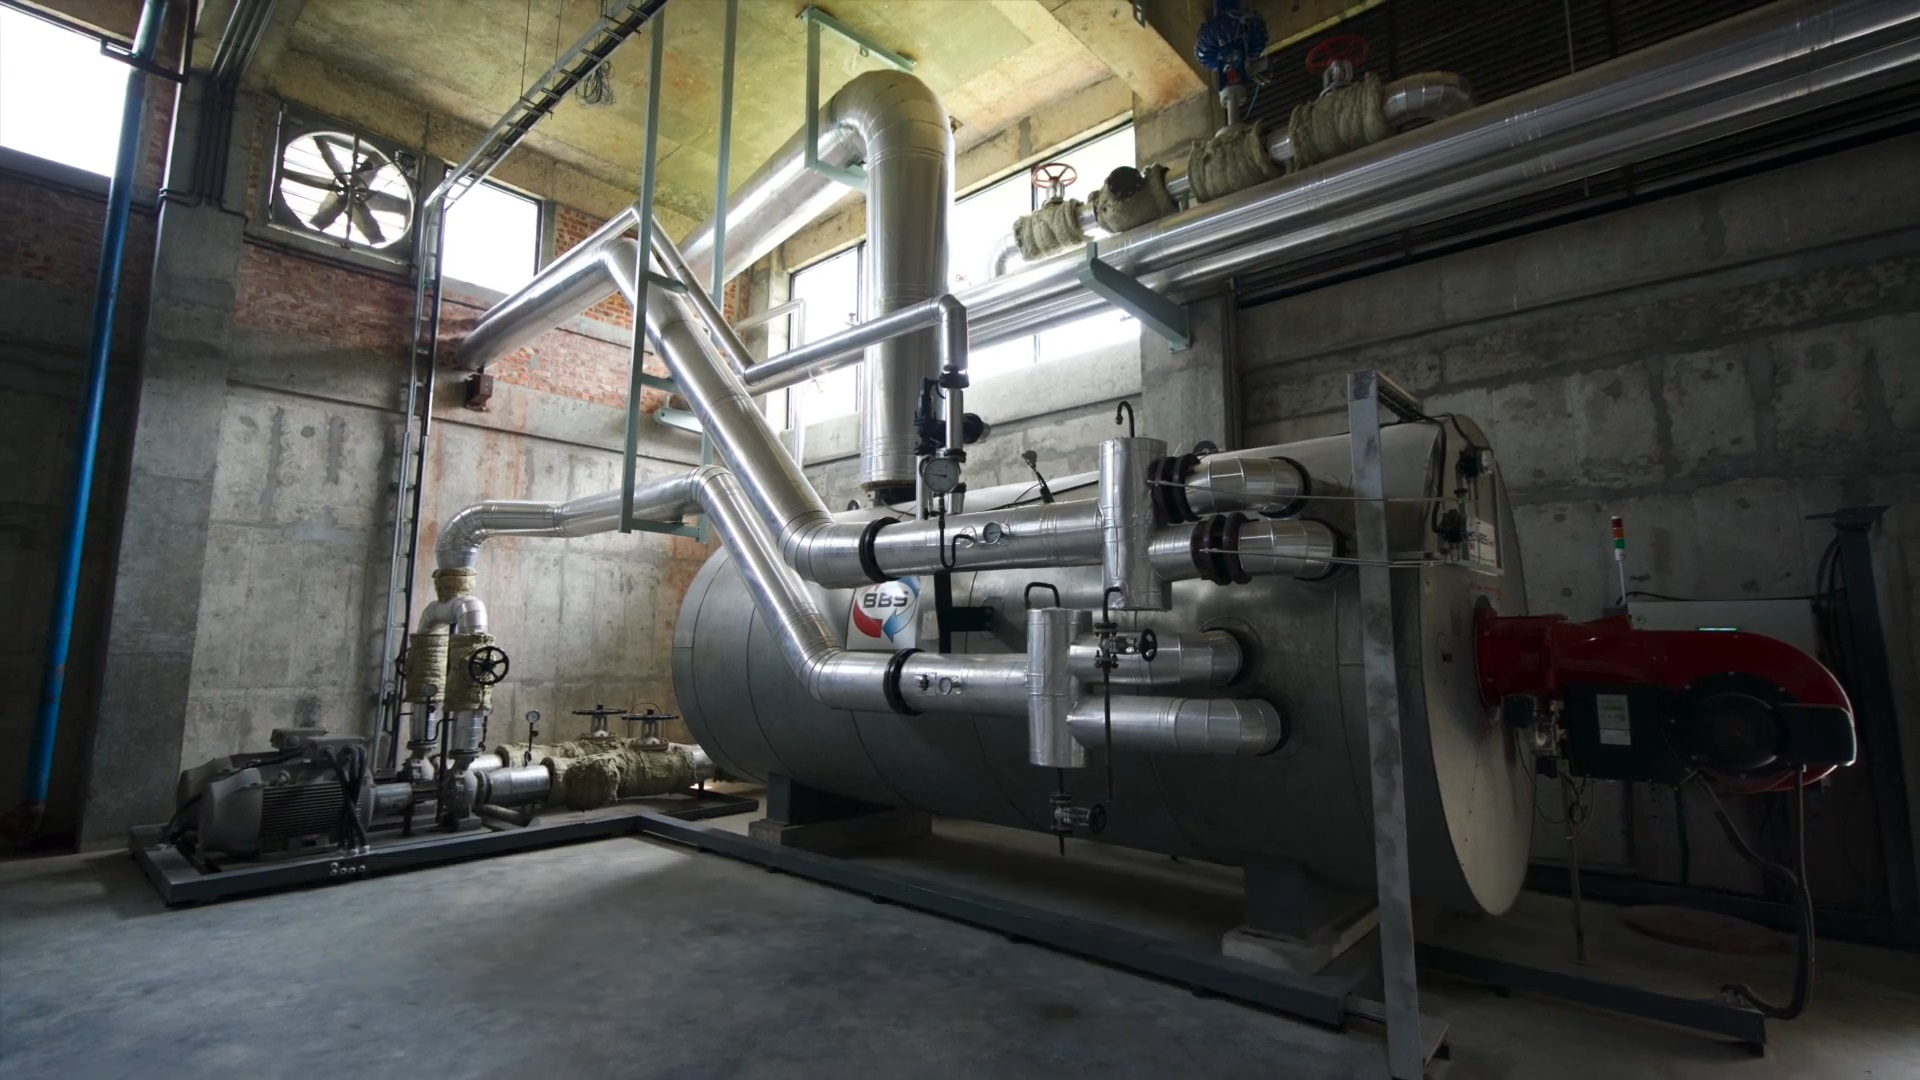
\includegraphics[width=0.8\linewidth]{figs/boiler.jpg}
    \caption{Boiler at Renaissance Apparel Ltd.}
    \label{fig:boiler}
\end{figure}
Boilers will be discussed in detail in the boilers chapter.

\newpage
\subsection{Technologies and Innovations}
Several technologies and innovations have been developed to improve the efficiency and sustainability of steam generation systems. These include:

\textbf{1. Combined Heat and Power (CHP):} Also known as cogeneration, CHP systems simultaneously produce electricity and useful heat from the same energy source, improving overall efficiency.

\textbf{2. Advanced Boiler Materials:} The development of high-temperature alloys and coatings enhances boiler efficiency and longevity, allowing for higher operating pressures and temperatures.

\textbf{3. Waste Heat Recovery:} Systems that capture and reuse waste heat from industrial processes or exhaust gases improve overall energy efficiency and reduce fuel consumption.

\textbf{4. Supercritical and Ultra-Supercritical }Boilers: These advanced boiler designs operate at pressures and temperatures above the critical point of water, resulting in higher thermal efficiencies and reduced emissions.

\subsection{Accessories for Steam Distribution System}

\subsubsection{Strainer}
A strainer valve is a type of pipe fitting used to purify, filter, or separate liquid from solids while still allowing the liquid to flow through it. Most often, strain is employed to remove steam from a stream of mixed liquids.

\subsubsection{Pipe}
A pipe transports pressurized steam from a boiler to the functional components, like the steam engine or turbine. Such piping generally incorporates valves to control the flow of the steam or to stop it entirely.

\subsubsection{Moisture Separator}
Air with moisture is sent from the cooler to the separator. The is twirled around in air. As it is accelerated through it, a diffuser propels the separator's body. rotating force causes water droplets to hit the separator wall, where they are then gravitationally collected.

\subsubsection{Thermodynamic Trap}
The thermodynamic trap is a steam trap that operates simply but is exceptionally long-lasting. The trap works by utilizing the dynamic action of flash steam as it passes through the trap.

\subsubsection{Ball Float Trap}
Traps having a wide range of uses. Condensate loads of any weight can be efficiently handled. little in scale. Because of the high and continuous discharge capacity, maximum heat transfer is guaranteed. A ball float steam trap is the best solution for draining plants with automatic temperature control.

\subsubsection{PRV}
In spite of changes in demand and/or upstream (inlet) water pressure, a pressure-reducing valve (PRV) is an automatic control valve created to reduce higher unregulated input pressure to a constant, reduced downstream (outlet) pressure.

\subsubsection{Safety Valve}
Steam systems typically employ safety valves for downstream pressure-reduction devices and boiler overpressure protection, among other uses. Safety valves are used in process operations to prevent product damage due to excessive pressure even though their primary purpose is to ensure safety.

\subsubsection{Deaerator Head}
The current boiler feed water tank now has a Deaerator Head addition that has mixing nozzles for new make-up water, flash steam, and plant area condensate. The stainless-steel perforated mixing pipe is immersed in feed water. This makes it possible for the feed water tank to uniformly mix hot condensate, flash steam, and make-up water.

\refstepcounter{figure}\addcontentsline{lof}{figure}{\protect\numberline{\thefigure}Organogram of Forbes Marshall}
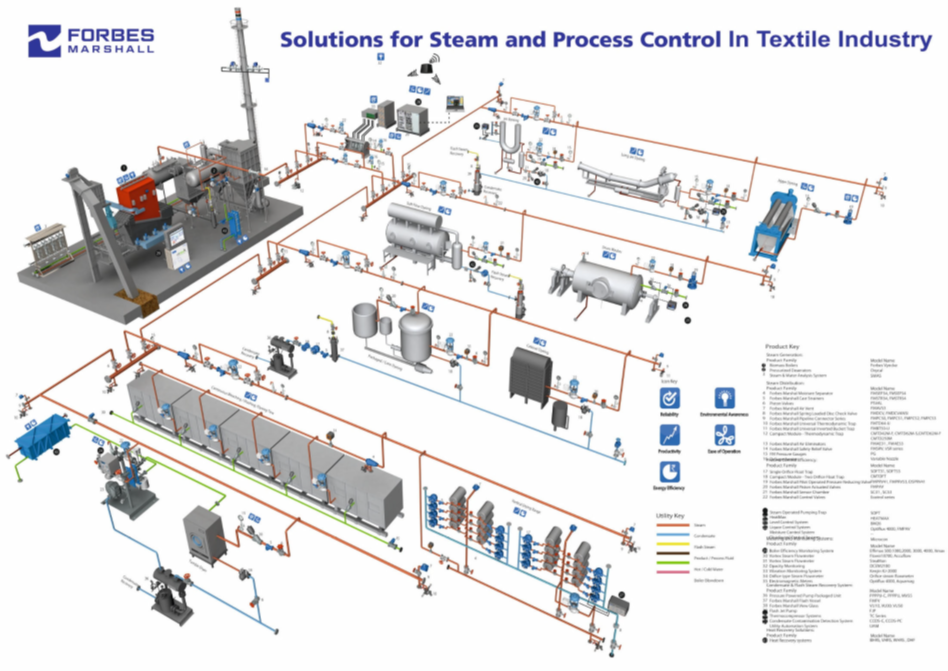
\includepdf[pages=-, angle=90]{chapters/gen_&_dist/steam_circuit_textile.pdf}
